\section{Laboratory work implementation}

\subsection{Tasks and Points}

I chose to implement the tasks for \textit{Normal Level}:
\begin{enumerate}
	\item Draw 5 lines of different colors and weights
	\item	Draw 2 Bezier curves
	\item	Draw 4 plane objects (ex. circle, square, pie, polygon...) of different colors, weights, filled and not
	\item	Draw 2 different objects using mouse
\item	Draw a Bezier curve using mouse
\item Clean with mouse.
\item Draw a custom bitmap image
\item Fill 2 object with gradient
\end{enumerate}

\subsection{Laboratory work analysis}

 \url{https://github.com/szraksy/WP}

I created a window and i put there 7 different buttons which are drawing Planes, Drawing lines, Drawing Bezier Curves,Drawing with mouse, generating bitmap, gradient and clearing all things.

When we click the drawing planes button then we will see there 4 different planes such rectangle, square, ellips and circle.

When we click the drawing lines then we can see there 5 different lines which are different colors and wieghts.

When we click the drawing bezier Curves button then we can see 2 different bezier curves.


When we click the draw with mouse button then a new popup windows will appeare there and we can draw lines with our mouse and also there is the another button down bellow the new window it works to do rectangle or squere by mouse.

When we click the Bitmap then its generating a bitmap file and it is writing file format.

When we click the Gradient then we will see the 4 different gradient planes.
	
When we click the clean button then all screen will be clean.
Also When we right click then will clear all secreen too.

On the white area we can draw a circle and bezier curve.


\subsection{Prove your work with screens}

\begin{figure}
	\centering
	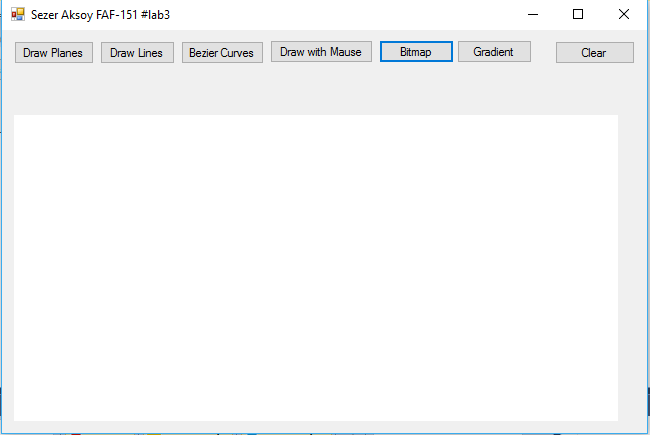
\includegraphics[width=0.7\linewidth]{../../LAB3/img/1}
	\caption{}
	\label{fig:1}
\end{figure}

\begin{figure}
	\centering
	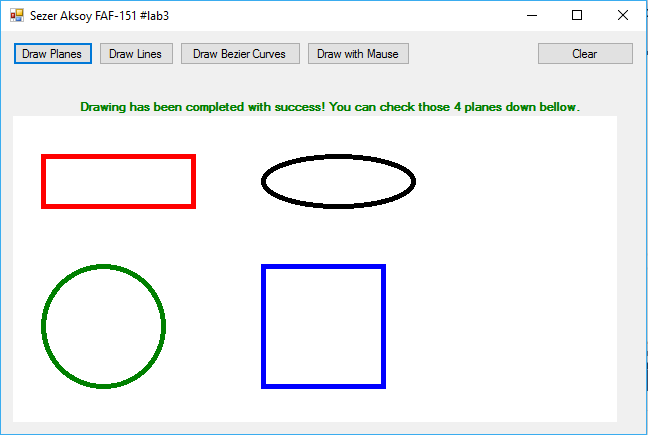
\includegraphics[width=0.7\linewidth]{../../LAB3/img/2}
	\caption{}
	\label{fig:2}
\end{figure}

\begin{figure}
	\centering
	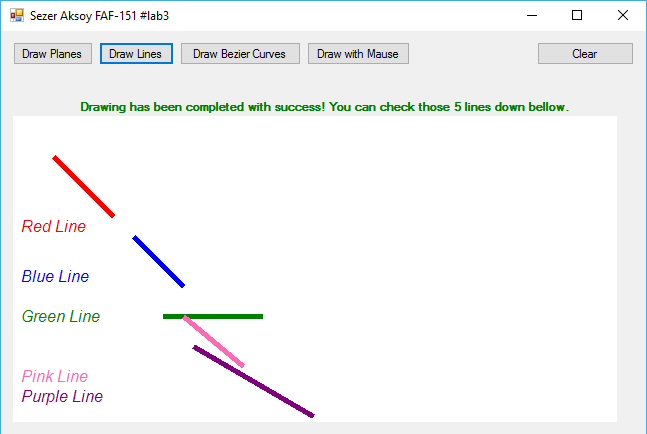
\includegraphics[width=0.7\linewidth]{../../LAB3/img/3}
	\caption{}
	\label{fig:3}
\end{figure}


\begin{figure}
	\centering
	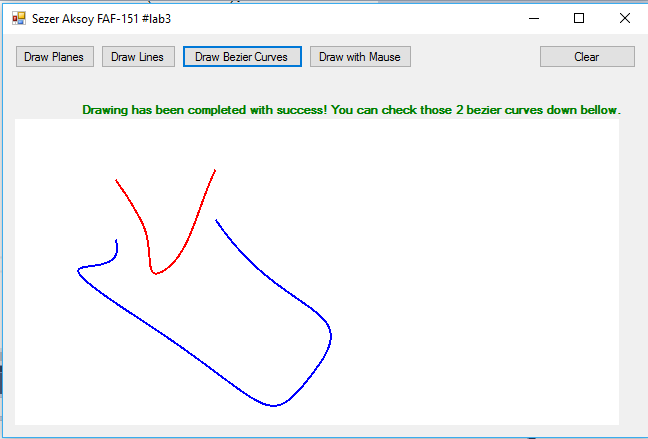
\includegraphics[width=0.7\linewidth]{../../LAB3/img/4}
	\caption{}
	\label{fig:4}
\end{figure}


\begin{figure}
	\centering
	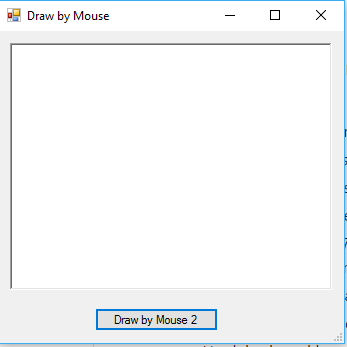
\includegraphics[width=0.7\linewidth]{../../LAB3/img/5}
	\caption{}
	\label{fig:5}
\end{figure}


\begin{figure}
	\centering
	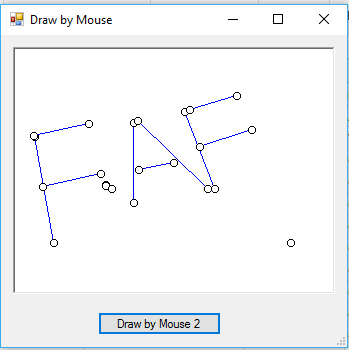
\includegraphics[width=0.7\linewidth]{../../LAB3/img/6}
	\caption{}
	\label{fig:6}
\end{figure}


\begin{figure}
	\centering
	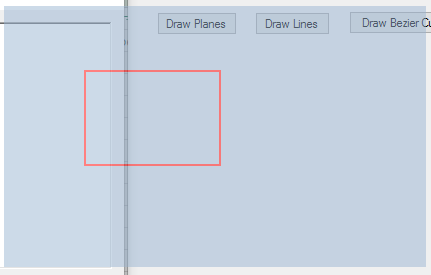
\includegraphics[width=0.7\linewidth]{../../LAB3/img/7}
	\caption{}
	\label{fig:7}
\end{figure}


\begin{figure}
	\centering
	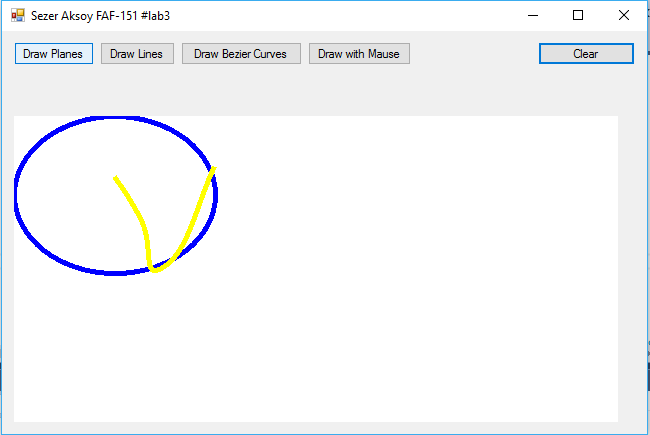
\includegraphics[width=0.7\linewidth]{../../LAB3/img/8}
	\caption{}
	\label{fig:8}
\end{figure}


\begin{figure}
	\centering
	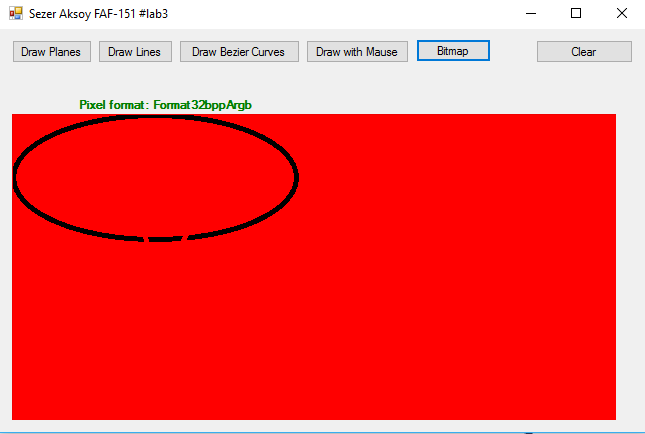
\includegraphics[width=0.7\linewidth]{../../LAB3/img/9}
	\caption{}
	\label{fig:9}
\end{figure}


\begin{figure}
	\centering
	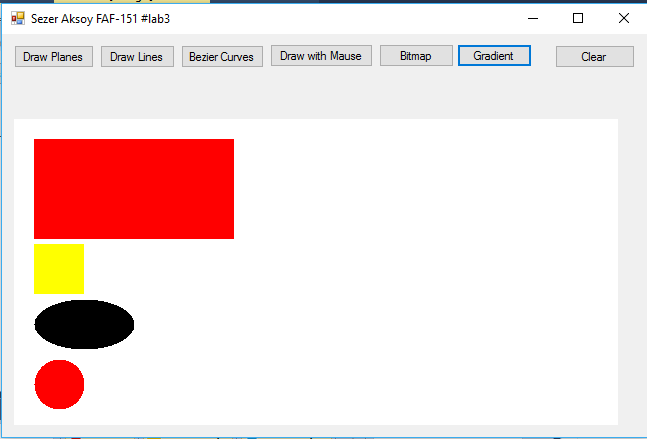
\includegraphics[width=0.7\linewidth]{../../LAB3/img/10}
	\caption{}
	\label{fig:10}
\end{figure}




\clearpage